\documentclass{article}
\usepackage{amsmath}
\usepackage{amssymb}
\usepackage{enumerate}
\usepackage{graphicx}
\usepackage{geometry}
\usepackage{enumitem}
\usepackage{xcolor}
\usepackage{tikz}
\usetikzlibrary{positioning}
\usepackage{amsmath}
\usepackage{nicematrix}
\usepackage{blindtext}
\usepackage{multicol}


\newcommand{\R}{\mathbb{R}}
\newcommand{\N}{\mathbb{N}}
\newcommand{\Z}{\mathbb{Z}}
\newcommand{\Q}{\mathbb{Q}}

\parindent 0in

\begin{document}

\noindent\textbf{Math 243 Discrete Mathematics \hfill Homework 6}

\begin{enumerate}
    \item In each question part below, I will list a set $\mathit{S}$ and 
    a rule that defines a relation $\mathit{R}$ on $\mathit{S}$ as follows: 
    $(\mathit{m,n}) \in R$ if $\mathit{m}$ and $\mathit{n}$ satisfy the given rule. 
    For each set and rule, do the following five things: 
%qustion 1
\begin{enumerate}[label=\bfseries \roman*]
\item List the order pairs in the relation.
\item Draw the associated arrow diagram.
\item Give the matrix representation of the relation. 
Be sure to label the rows and columns with the elements of $S$.
\item Identify which properties the relation has: reflexive, 
antireflexive, or neither; symmetric, antisymmetric, or neither; 
transitive or not transitive. Be sure to explain your answers.
\item Decide whether the relation is an equivalence relation. 
If so, identify the equivalence classes.     
\end{enumerate}

\begin{enumerate}
    \item $\mathit{S}$ = \{4,9,17\}; $m \geq n$.    
    \item $\mathit{S}$ = \{0,2,5\}; $mn$ = 0.
    \item $\mathit{S}$ = \{1,2,6,7,11\}; $m \equiv n \pmod{3}$
\end{enumerate}

%answer to question 1
\small
\underline{Answers for (a):}    

\begin{itemize}
    \item R = \{$(m,n):m \geq n$ and $m,n \in S$\}
    \\$\Rightarrow$ \{(17,4),(9,4),(17,9),(4,4),(9,9),(17,17)\}\\
   
    \begin{multicols}{2}
        \item Diagram:\\
        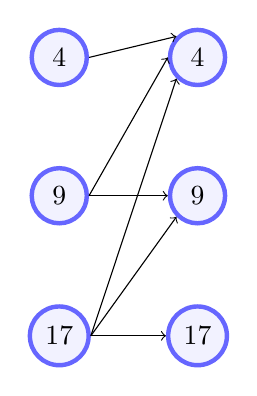
\begin{tikzpicture}[roundnode/.style={circle, draw=blue!60, fill=blue!5, ultra thick, minimum size=7mm},]
            %Nodes
            \node[roundnode](maintopic){4};
            \node[roundnode](rightcirlce_4)[right=of maintopic]{4};
            \node[roundnode](rightcirlce_9)[below=of rightcirlce_4]{9};
            \node[roundnode](rightcirlce_17)[below=of rightcirlce_9]{17};
            \node[roundnode](leftcirlce_9)[below=of maintopic]{9};
            \node[roundnode](leftcirlce_17)[below=of leftcirlce_9]{17};
            
            %Lines
            \draw[->] (maintopic.east) -- (rightcirlce_4.north west);
            \draw[->] (leftcirlce_9.east) -- (rightcirlce_4.west);
            \draw[->] (leftcirlce_9.east) -- (rightcirlce_9.west);
            \draw[->] (leftcirlce_17.east) -- (rightcirlce_4.south west);
            \draw[->] (leftcirlce_17.east) -- (rightcirlce_9.south west);
            \draw[->] (leftcirlce_17.east) -- (rightcirlce_17.west);
        \end{tikzpicture}
        \columnbreak
        \item Matrix:\\
            $\begin{pNiceMatrix}[first-row,first-col]
            & 4 & 9 & 17          \\
            4  & 1 & 0 & 0        \\ 
            9  & 1 & 1 & 0        \\
            17 & 1 & 1 & 1        \\
            \end{pNiceMatrix}$
            Matrix = 
            $\begin{cases}
                1: (m,n)\in R\\
                0: otherwise\\  
            \end{cases}$ \\

        \item \begin{itemize}
        \item R is reflexive as $(m,n) \in R$ $\forall$ $m \in S$
        \item R is anti symmetric. As if(a,b) $\in R$ and (b,a) $\in R$ then a = b for: 
            \begin{itemize}
                \item[] a = b = 4 
                \item[] a = b = 9 
                \item[] a = b = 17
            \end{itemize}
            \item R is transitive. As if (a,b)$\in R$ and (b,c)$\in R$ then (a,c)$\in R$ holds. $\therefore a,b,c \in S$  
        \end{itemize}
        \item R is not an equivalence relation based on the reasons mentioned above.
    \end{multicols} 
\end{itemize}

\pagebreak %-------------------------------------------------------------------------------------------

\underline{Answers for (b):}    

\begin{itemize}
    \item R = \{$(m,n):mn = 0$ and $m,n \in S$\}
    \\$\Rightarrow$ \{(0,0),(0,2),(0,5),(2,0),(5,0)\}\\
\begin{multicols}{2}
    \item Diagram:\\
    \begin{tikzpicture}[roundnode/.style={circle, draw=blue!60, fill=blue!5, ultra thick, minimum size=7mm},]
        %Nodes
        \node[roundnode](maintopic){0};
        \node[roundnode](rightcirlce_0)[right=of maintopic]{0};
        \node[roundnode](rightcirlce_2)[below=of rightcirlce_0]{2};
        \node[roundnode](rightcirlce_5)[below=of rightcirlce_2]{5};
        \node[roundnode](leftcirlce_2)[below=of maintopic]{2};
        \node[roundnode](leftcirlce_5)[below=of leftcirlce_9]{5};
        
        %Lines
        \draw[->] (maintopic.east) -- (rightcirlce_0.west);
        \draw[->] (maintopic.east) -- (rightcirlce_2.west);
        \draw[->] (maintopic.east) -- (rightcirlce_5.west);
        \draw[->] (leftcirlce_2) -- (rightcirlce_0.south west);
        \draw[->] (leftcirlce_5) -- (rightcirlce_0.south);

    \end{tikzpicture}

    \item Matrix:\\
        $\begin{pNiceMatrix}[first-row,first-col]
           & 0 & 2 & 5        \\
        0  & 1 & 1 & 1        \\ 
        2  & 1 & 0 & 0        \\
        5  & 1 & 0 & 0        \\
        \end{pNiceMatrix}$
        Matrix = 
        $\begin{cases}
            1: mn = 0 \\
            0: otherwise\\  
        \end{cases}$ \\

    \item \begin{itemize}
       \item R is not reflexive as $(2,2) \notin R$ 
       \item R is symmetric as (0,2) $\in R$ and (2,0) $\in R$
        \item R is not transitive. Because (2,0) and (0,5) $\in R$ but (2,5) $\notin R$  
     \end{itemize}
    \item R is not an equivalence relation based on the reasons mentioned above.
\end{multicols}
    
\end{itemize}

\underline{Answers for (c):}    

\begin{itemize}
    \item R = \{(m,n): $m \equiv n \pmod{3}$ and $m,n \in S$\}
    \\$\Rightarrow$ \{(1,1),(2,2),(6,6),(7,7),(11,11),(1,7),(7,1),(2,11),(11,2)\}
    \begin{multicols}{2}
        \item Diagram:\\
        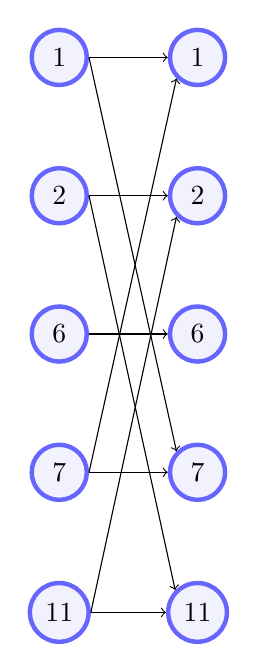
\begin{tikzpicture}[roundnode/.style={circle, draw=blue!60, fill=blue!5, ultra thick, minimum size=7mm},]
            %Nodes
            \node[roundnode](maintopic){1};
            \node[roundnode](leftcirlce_2)[below= of maintopic]{2};
            \node[roundnode](leftcirlce_6)[below= of leftcirlce_2]{6};
            \node[roundnode](leftcirlce_7)[below= of leftcirlce_6]{7};
            \node[roundnode](leftcirlce_11)[below= of leftcirlce_7]{11};
            \node[roundnode](rightcirlce_1)[right= of maintopic]{1};
            \node[roundnode](rightcirlce_2)[below= of rightcirlce_1]{2};
            \node[roundnode](rightcirlce_6)[below= of rightcirlce_2]{6};
            \node[roundnode](rightcirlce_7)[below= of rightcirlce_6]{7};
            \node[roundnode](rightcirlce_11)[below= of rightcirlce_7]{11};

            %Lines
            \draw[->](maintopic.east)--(rightcirlce_1.west);
            \draw[->](maintopic.east)--(rightcirlce_7.north west);
            \draw[->](leftcirlce_2.east)--(rightcirlce_2.west);
            \draw[->](leftcirlce_2.east)--(rightcirlce_11.north west);
            \draw[->](leftcirlce_6.east)--(rightcirlce_6.west);
            \draw[->](leftcirlce_7.east)--(rightcirlce_1.south west);
            \draw[->](leftcirlce_7.east)--(rightcirlce_7.west);
            \draw[->](leftcirlce_11.east)--(rightcirlce_2.south west);
            \draw[->](leftcirlce_11.east)--(rightcirlce_11.west);


        \end{tikzpicture}
        \item Matrix:\\
            $\begin{pNiceMatrix}[first-row,first-col]
               & 1 & 2 & 6 & 7 & 11  \\
            1  & 1 & 0 & 0 & 1 & 0   \\ 
            2  & 0 & 1 & 0 & 0 & 1   \\
            6  & 0 & 0 & 1 & 0 & 0   \\
            7  & 1 & 0 & 0 & 1 & 0   \\
            11 & 0 & 1 & 0 & 0 & 1   \\
            \end{pNiceMatrix}$
            Matrix = 
            $\begin{cases}
                1: m \equiv n \pmod{3}\\
                0: otherwise\\  
            \end{cases}$ \\

        \item \begin{itemize}
            \item R is reflexive as the diagnol of the matrix consist on only 1's.
            \item R is symmetric as since $\forall$ $m$ and $n$, (m,n) and (n,m) are 1's.
            \item R is transitive as $\forall$ $m$ and $n \in R$, if $mRn$ and $nRm$ 
            then $mRm$ and $nRn$.
        \end{itemize}
        \item R is an equivalence relation since it is reflexive,symmetric, and transitive for 
        the reasons mentioned above.
    \end{multicols}
\end{itemize}


\pagebreak %-------------------------------------------------------------------------------------------

%question 2

    \item Suppose $X$ is the set \{$a,b,c,d,e$\} and $P(X)$ is the power set of $X$. 
    The domain of each of the relations below is $P(X)$. 
    For each relation, describe the relation in words. Then determine whether it is 
    reflexive, antireflexive, or neither; symmetric, anti-symmetric, or neither; and 
    transitive or not transitive.
\begin{multicols}{2}
    \begin{enumerate}
        \item $A$ is related to $B$ if $\lvert A-B \rvert$ = 1. The 
        vertical bars mean the cardinality of $A - B$.
        \begin{enumerate}

            \item Let $A \in P(X)$:\\
                $\Rightarrow$ Now, $A - A$ = $\emptyset$\\
                $\Rightarrow$ $\left\lvert A - A\right\rvert$ = 0 $\neq 1$\\
                $\Rightarrow$ $A \nsim A$.\\
                Since the choice of set A is completely arbritiary, we can say that set $A$ is 
                $\textbf{anit-reflexive.}$\\

            \item Let $A$ = \{a\}, $B$ = $\emptyset$ and $A,B \in P(X)$:\\
                $\Rightarrow$ $A-B$ = \{a\} and $B-A$ = $\emptyset$\\
                $\Rightarrow$ $\left\lvert A - B\right\rvert$ = 1 and $\left\lvert B - A\right\rvert$ = 0\\
                $\Rightarrow$ From this we can say that $A \sim B$ but $B \nsim A$\\
                This results in the conclusion that the relation is $\textbf{not symmetric}$.\\

            \item Let $A$ = \{a,b\}, $B$ = {b,a} and $A,B \in P(X)$:\\
                $\Rightarrow$ $A-B$ = \{a\} and $B-A$ = \{c\} \\
                $\Rightarrow$ $\left\lvert A - B\right\rvert$ = 1 and $\left\lvert B - A\right\rvert$ = 1\\
                $\Rightarrow$ From this we can say that $A \sim B$ and $B \sim A$ but $A \neq B$\\
                We can say that the relation is not antisymmetric. $\therefore$ The relation is 
                $\textbf{neiter symmetric nor antisymmetric}$.\\

            \item Let $A$ = \{a,b\}, $B$ = {b,c} and $A,B \in P(X)$:\\
                $\Rightarrow$ $A-B$ = \{a\} and $B-A$ = \{c\} \\
                $\Rightarrow$ $\left\lvert A - B\right\rvert$ = 1 and $\left\lvert B - A\right\rvert$ = 1\\
                $\Rightarrow$ From this we can say that $A \sim B$ and $B \sim A$\\
                But from the (i) we said that $A \nsim A$,\\ $\therefore$ The relation is $\textbf{not transitive}$.
        \end{enumerate}

    In short, the relation is :
    \begin{itemize}
        \item $\textbf{antireflexive}$
        \item $\textbf{neither symmetric and anti-symmetric}$
        \item $\textbf{not transitive}$
    \end{itemize}
    
    \columnbreak
    
    \item $A$ is related to $B$ if $A \subset B$. Note 
        that this notation means proper subset.
        \begin{enumerate}
            \item Since every element of a set $A$ is contained in itself, $A \sim A$ $\forall A$
            and it makes the relation $\textbf{reflexive}$\\
            \item Let $A \sim B$ and $B \sim A$. Here as per definition, every element of $A \in B$ 
            and  $B \in A$ also. Hence A = B. \\$\therefore$ The relation is $\textbf{antisymmetric}$.\\
            \item  Let $A \sim B$ and $B \sim C$, then it means that $A \in B$ and $B \in C$. That automatically puts 
            every element of A inside C. So $A \sim C$ and hence the relation is $\textbf{transitive}$.\\
        \end{enumerate}
        In short, the relation is :
    \begin{itemize}
        \item $\textbf{reflexive}$
        \item $\textbf{antisymmetric}$
        \item $\textbf{transitive}$
    \end{itemize}
    \end{enumerate}
\end{multicols}
\pagebreak %-------------------------------------------------------------------------------------------

%question 3
\item Determine whether the following relations are equivalence relations. 
If so, show that the relation fulfills the requirements for an equivalence relation, 
and describe the equivalence classes. If not, show how the relation fails to fulfill 
the requirements.

\begin{enumerate}
    \item The relation $\mathcal{C}$ is defined by $(x,y)\in \mathcal{C}$ iff cos($x$) = cos($y$), 
    where $x,y \in \R$.
    \begin{itemize}
        \item Reflexive:\\ Let $y = x$. From this, $(x,x) \in \mathcal{C}$.\\ 
        $\Rightarrow$ $\therefore$ cos($x$) = cos($x$) holds.\\
        Similarly, let $x = y$. From this $(y,y)$\\ 
        $\Rightarrow$ $\therefore$ cos($y$) = cos($y$) also holds.\\$\textbf{Reflexivity holds.}$\\

        \item Symmetric:\\If $x \sim y$, then it implies that $y \sim x$.\\Assume that $(x,y) \in 
        \mathcal{C}$ then cos($x$) = cos($y$) can be rewritten as cos($y$) = cos($x$).\\This implies 
        that $(y,x) \in \mathcal{C}$.\\$\textbf{Symmetry holds.}$\\ 

        \item Transitivity:\\If $(x,y) \in \mathcal{C}$ and $(y,z) \in \mathcal{C}$, then $(x,z) \in \mathcal{C}$.\\
        Assume that $(x,y) \in \mathcal{C}$, $(y,z) \in \mathcal{C}$.$\therefore$\\
        cos($x$) = cos($y$)\\
        cos($y$) = cos($z$)\\
        This implies that cos($x$) = cos($z$) and $(x,z) \in \mathcal{C}$.\\$\textbf{Transitivity holds.}$\\
    \end{itemize}
    Therefore, it is an equivalence relation. The equivalence classes are:\\
    $\rightarrow$ If $a \in \R$, the equivalence classes will be $[a]$ = \{$x \in \R$: cos($a$) = cos($x$)\}\\

    \item The relation $\varpropto$ on the domain $\Z^+\times\Z^+$ is defined by $(m,n) \varpropto (p,q)$ iff $mq = np$.
    \begin{itemize}
        \item Reflexive:\\Let $n = m$ and $q = p$. Then $(m,m) \in \Z^+\times\Z^+$ iff $mp = mp$\\$\therefore$ $\textbf{Reflexivity holds.}$\\
        \item Symmetric:\\If $(m,n)$ and $(p,q)$ are related then it implies $(p,q)$ and $(m,n)$ are related.\\Assume that $(m,n) \varpropto (p,q)$,
        this says that $mq = np$ and can be rewritten as $qm = pn$. This says, $(q,p) \sim (m,n)$\\$\therefore$ $\textbf{Symmetry does not hold.}$
    \end{itemize}

    Because symmetry does not hold, the relation is $\textbf{not an equivalence relation.}$ The reason for this conclusion is soley
    because as long as a relation does not hold at least one of the requirements, the relation fails to be an equivalence relation. In this case,
    we dont not need to prove or disprove transitivity since symmetry already failed.
\end{enumerate}

\end{enumerate}

\end{document}